% 软件  软件分析
%作者:赵启
%上次更新:2020年1月10日 17:20


\chapter{软件分析}

\section{综述}

  {\songti 在整个项目的设计与之后的装配分析中,我们均学习探索并使用了一些软件进行辅助性分析,
 这对于我们进行相关的材料选择、整体设计、寿命分析以及装配的整体合理性都有了很大的帮助。}

 


  \newpage

\section{基于ROS环境的机械臂分析}

{\songti 为了更好地去分析整个装置,我们小组尝试了Robot Operating System机器人操控系统(以下简称ROS),首先,我们下载安装了了Ubuntu系统,并在Ubuntu系统上搭建ROS环境和相关的功能包,之后在SolidWorks软件中搭建六自由度机械臂的坐标系体系,使用sw urdf exporter
 插件生成了通用机器人描述文件(URDF),成功地把我们设计的模型导入进入了ROS系统。

{\songti 通过ROS环境中模拟出的模型,我们获得了机械臂运动的包络面和模拟路径。并通过后续的学习可以了解到在ROS环境中可以实现电控,但由于时间和精力有限所以小组准备在寒假进行进一步探索。}

\begin{figure}[!htp]
  \centering
  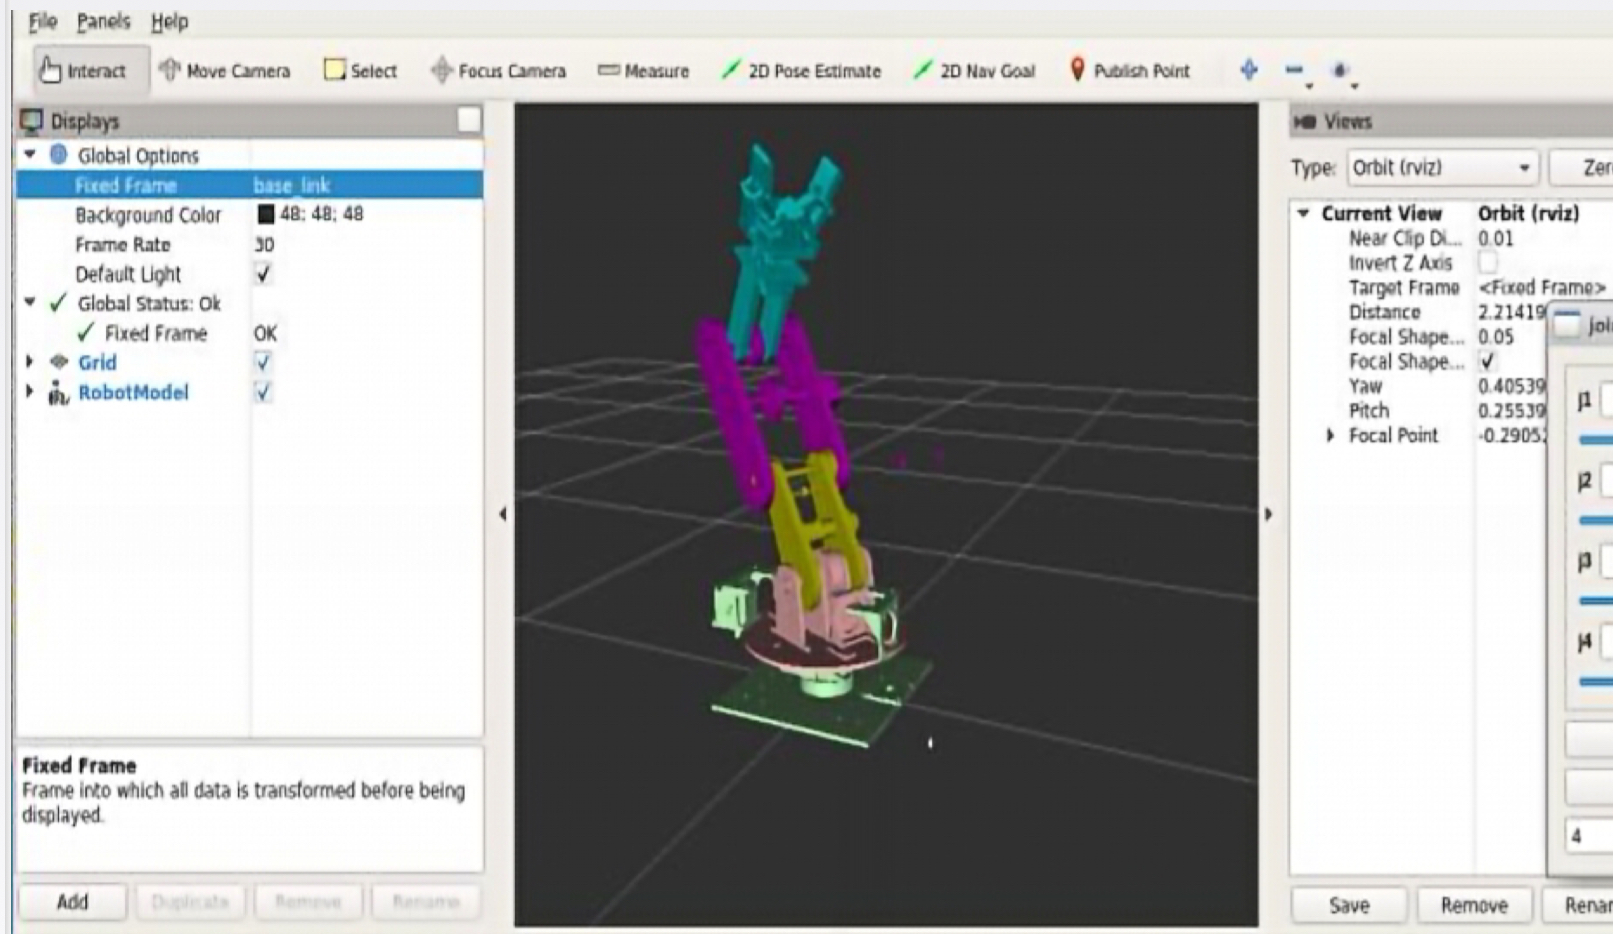
\includegraphics[width=12cm]{ros_environment_setup.jpg}
  \bicaption[ROS环境搭建]{ROS环境搭建}{ROS environment construction}
  \label{fig:ROS环境搭建}
\end{figure}